\documentclass[11pt]{article}
\usepackage[a4paper,margin=1in]{geometry}
\usepackage{amsmath,amssymb,mathtools}
\usepackage{siunitx}
\usepackage{booktabs}
\usepackage{array}
\usepackage{graphicx}
\usepackage{longtable}
\usepackage{hyperref}
\usepackage{enumitem}
\usepackage{xcolor}

\graphicspath{{time_domain_fit_derivation_figures/}}

\title{THzSim2 Time-Domain Fitting and Oblique-Incidence Optical Response}
\author{THzSim2 Repository}
\date{\today}

\begin{document}
\maketitle

\section{Purpose and Scope}
This note documents the calculations used by the current \texttt{thzsim2} code path for
\begin{enumerate}[leftmargin=2em]
\item building a physical sample stack from notebook-facing layer definitions,
\item computing the sample optical response at arbitrary angle of incidence for explicit
\texttt{s} or \texttt{p} polarization,
\item propagating a measured or generated reference trace through that response, and
\item fitting unknown sample parameters directly in the time domain.
\end{enumerate}

The present implementation is intentionally scoped to \textbf{isotropic scalar multilayers}.
It does not model birefringence, anisotropy, Jones-matrix polarization conversion, or a full
ellipsometric instrument train. The measured reference trace is treated as the source term of
the forward model, so PCA emission, detector response, and any common-path optics outside the
sample are absorbed into that measured reference.

\section{Code Path Overview}
The end-to-end notebook path is
\[
\texttt{generate\_reference\_pulse / load\_reference\_csv}
\;\rightarrow\;
\texttt{prepare\_reference}
\;\rightarrow\;
\texttt{build\_sample}
\;\rightarrow\;
\texttt{simulate\_sample\_from\_reference}
\;\rightarrow\;
\texttt{fit\_sample\_trace}.
\]

The core implementation is distributed over these modules:
\begin{itemize}[leftmargin=2em]
\item \texttt{thzsim2/core/fft.py}: Fourier transform convention and inverse transform.
\item \texttt{thzsim2/core/materials.py}: dielectric functions and passive
$\tilde{n}=n+i k$ extraction.
\item \texttt{thzsim2/core/transfer.py}: Fresnel coefficients, oblique propagation,
single-layer Fabry--Perot sums, direct-interface handling, and arbitrary multilayer recursion.
\item \texttt{thzsim2/core/forward.py}: measurement normalization and
$E_{sam}(\omega)$ construction from the measured reference.
\item \texttt{thzsim2/core/fitting.py}: parameter mapping, objective evaluation,
optimization, and local covariance estimation.
\item \texttt{thzsim2/workflows/sample\_workflow.py}: notebook-facing sample resolution.
\item \texttt{thzsim2/workflows/reference.py}: notebook-facing reference workflow.
\end{itemize}

\section{Reference Trace and Fourier Convention}
\subsection{Time axis and trace}
Let the uniformly sampled reference trace be
\[
E_n = E(t_n),
\qquad
t_n = t_0 + n \Delta t,
\qquad
n=0,\dots,N-1.
\]
The reference may come from \texttt{generate\_reference\_pulse(...)} or from a measured CSV
imported by \texttt{load\_reference\_csv(...)} and normalized/exported by
\texttt{prepare\_reference(...)}.

\subsection{Forward transform}
\texttt{fft\_t\_to\_w(trace, dt, t0)} in \texttt{thzsim2/core/fft.py} computes
\[
\omega_k = 2\pi f_k,
\]
on the standard FFT angular-frequency grid returned by \texttt{make\_omega\_grid}, and
\[
\hat{E}(\omega_k)
=
\Delta t \, N \,
\operatorname{IFFT}(E_n)
\exp(i \omega_k t_0).
\]
The explicit $t_0$ factor is important because measured traces are usually not centered at
zero time.

\subsection{Inverse transform}
\texttt{ifft\_w\_to\_t(spectrum, dt, t0)} applies
\[
E_n
=
\frac{1}{N \Delta t}
\operatorname{FFT}
\left[
\hat{E}(\omega_k)\exp(-i\omega_k t_0)
\right].
\]
This pair is the exact convention used by the forward model and the time-domain fitter.

\begin{figure}[htbp]
\centering
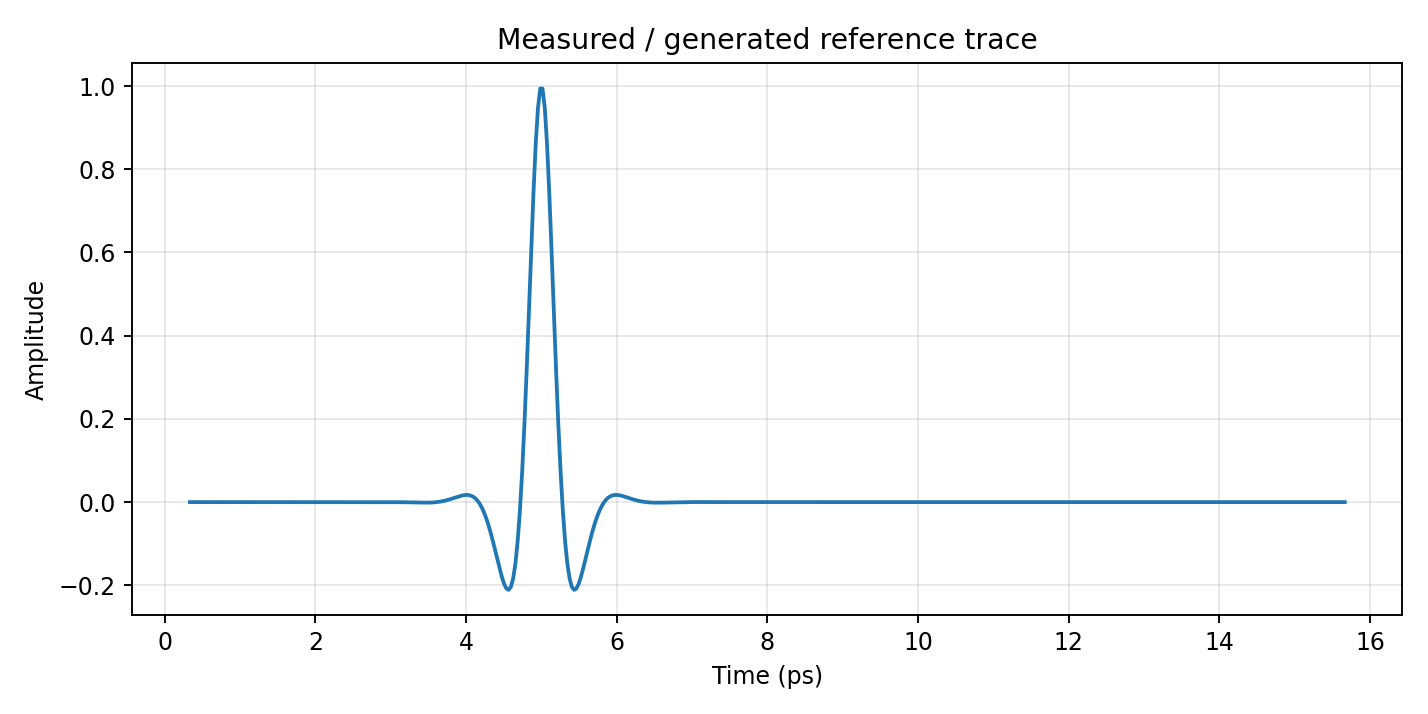
\includegraphics[width=0.82\linewidth]{transmission_reference_trace.png}
\caption{Reference trace generated by the documentation figure script. This is the waveform
that enters the forward model before the sample response is applied.}
\end{figure}

\begin{figure}[htbp]
\centering
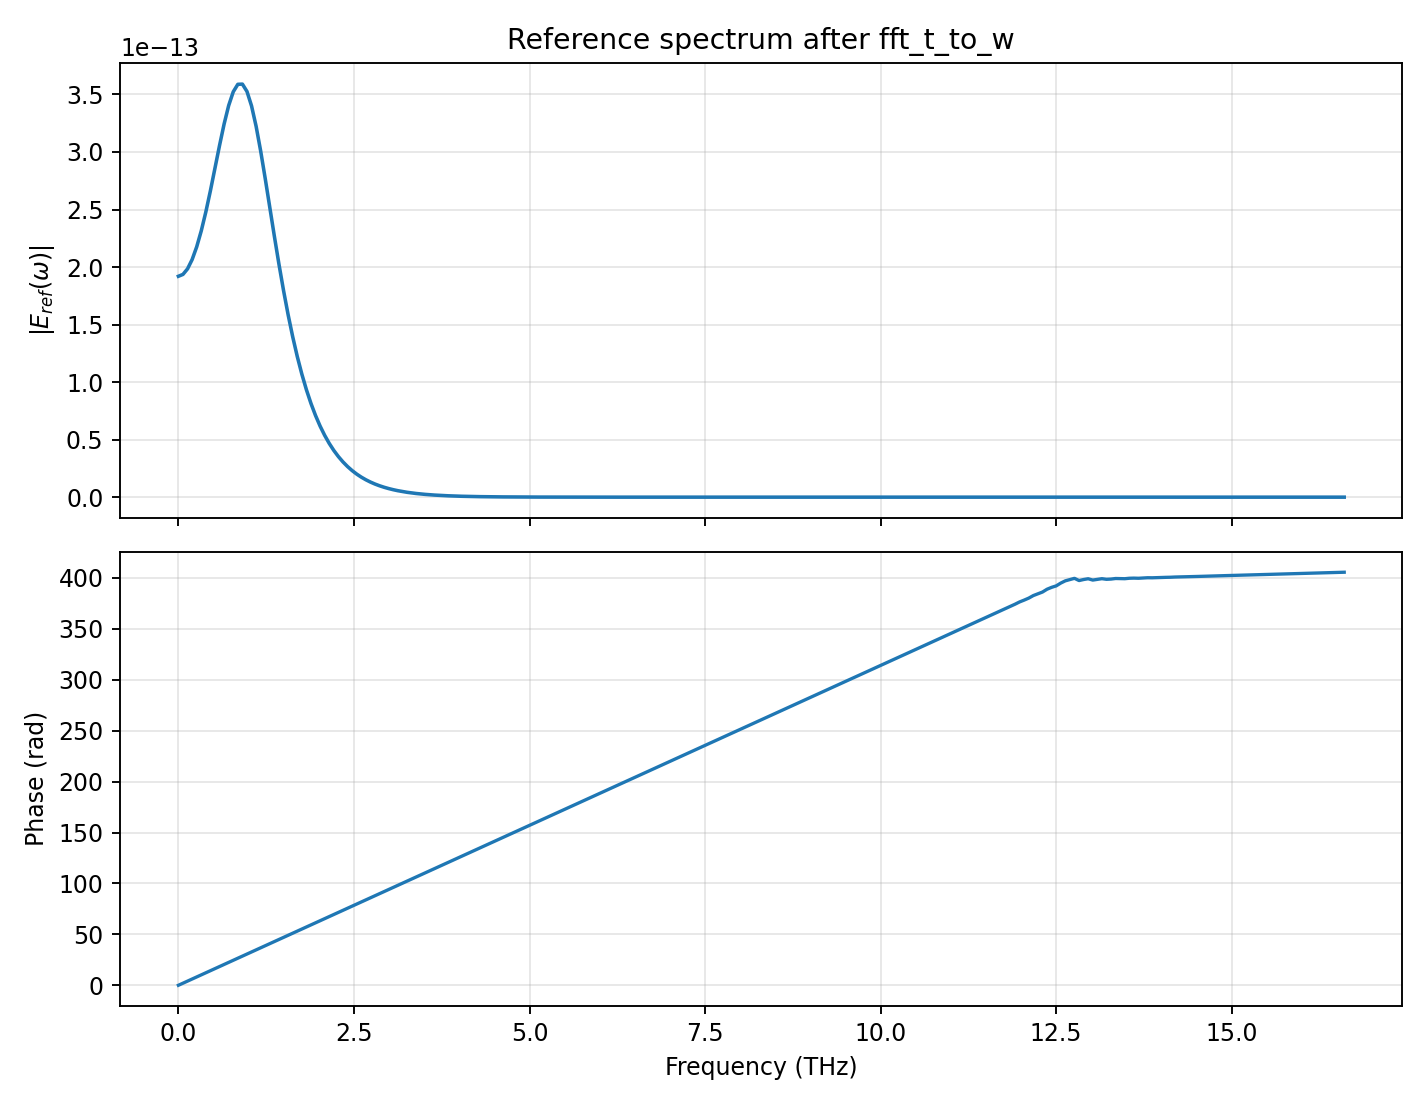
\includegraphics[width=0.82\linewidth]{transmission_reference_spectrum.png}
\caption{Magnitude and unwrapped phase of the reference spectrum after
\texttt{fft\_t\_to\_w}.}
\end{figure}

\section{Sample Resolution and Material Models}
\subsection{Notebook-facing layer definitions}
\texttt{build\_sample(...)} accepts notebook objects such as
\texttt{Layer}, \texttt{ConstantNK}, \texttt{Drude}, \texttt{Lorentz}, and
\texttt{DrudeLorentz}. The helper \texttt{\_resolve\_value(...)} in
\texttt{sample\_workflow.py} converts each scalar or \texttt{Fit(...)} entry into
\begin{enumerate}[leftmargin=2em]
\item a concrete initial parameter value stored in the resolved stack, and
\item an entry in \texttt{sample.fit\_parameters} when the quantity is a fit variable.
\end{enumerate}

If a fit parameter is declared on a material field such as
\texttt{layers[0].material.gamma\_thz}, the fitter maps it into the resolved stack by the path
conversion implemented in \texttt{stack\_path\_from\_user\_path(...)} and
\texttt{apply\_fit\_values(...)}.

\subsection{Dielectric functions}
The material models in \texttt{thzsim2/core/materials.py} are
\[
\varepsilon_{\text{Drude}}(\omega)
=
\varepsilon_\infty
- \frac{\omega_p^2}{\omega(\omega+i\gamma)},
\]
\[
\varepsilon_{\text{Lorentz}}(\omega)
=
\varepsilon_\infty
+
\Delta\varepsilon
\frac{\omega_0^2}{\omega_0^2-\omega^2-i\gamma\omega},
\]
and
\[
\varepsilon_{\text{Drude-Lorentz}}(\omega)
=
\varepsilon_\infty
- \frac{\omega_p^2}{\omega(\omega+i\gamma)}
+
\sum_m
\Delta\varepsilon_m
\frac{\omega_{0,m}^2}{\omega_{0,m}^2-\omega^2-i\gamma_m\omega}.
\]

The complex refractive index is obtained by
\[
\tilde{n}(\omega) = n(\omega) + i k(\omega) = \sqrt{\varepsilon(\omega)},
\]
with the passive branch selected by \texttt{nk\_from\_eps(...)} so that
\[
k(\omega) \ge 0.
\]

\subsection{Imported refractive-index files}
For \texttt{NKFile}, \texttt{build\_sample(...)} loads a \texttt{freq\_thz,n,k} CSV and uses
\texttt{\_linear\_interp\_extrap(...)} and \texttt{\_resolve\_imported\_nk(...)} to align the
tabulated $n,k$ values to the working positive-frequency grid.

\section{Oblique-Incidence Optics}
\subsection{Measurement configuration}
The measurement state is represented by the notebook-facing dataclasses
\texttt{Measurement} and \texttt{ReferenceStandard} in
\texttt{thzsim2/models/measurement.py}. The public fields are
\begin{itemize}[leftmargin=2em]
\item \texttt{mode}: \texttt{\"transmission\"} or \texttt{\"reflection\"},
\item \texttt{angle\_deg}: incidence angle in the incident medium,
\item \texttt{polarization}: \texttt{\"s\"} or \texttt{\"p\"},
\item \texttt{reference\_standard}: either \texttt{identity} or an explicit stack.
\end{itemize}

\subsection{Tangential-wavevector conservation and branch choice}
For an isotropic stack, the tangential component of the wavevector is conserved. If the
incident medium is $\tilde{n}_0$ and the incidence angle is $\theta_0$,
\[
\tilde{n}_j \sin\theta_j = \tilde{n}_0 \sin\theta_0.
\]
The code works with
\[
\tilde{n}_{\parallel} = \tilde{n}_0 \sin\theta_0,
\qquad
\cos\theta_j
=
\sqrt{1-\left(\frac{\tilde{n}_{\parallel}}{\tilde{n}_j}\right)^2}.
\]
Because $\tilde{n}_j$ can be complex, the square root has two branches. The helper
\texttt{\_forward\_cos\_theta(...)} chooses the branch for which the normal propagation factor
\[
\tilde{n}_j \cos\theta_j
\]
corresponds to a forward-decaying or forward-propagating wave:
\[
\Im\!\left(\tilde{n}_j \cos\theta_j\right) \ge 0,
\]
and if the imaginary part is numerically zero it also requires
\[
\Re\!\left(\tilde{n}_j \cos\theta_j\right) \ge 0.
\]

\subsection{Oblique Fresnel coefficients}
For the interface from medium $j$ to medium $k$, \texttt{fresnel\_t\_oblique(...)} and
\texttt{fresnel\_r\_oblique(...)} use
\[
t^{(s)}_{jk}
=
\frac{2 \tilde{n}_j \cos\theta_j}
{\tilde{n}_j \cos\theta_j + \tilde{n}_k \cos\theta_k},
\qquad
r^{(s)}_{jk}
=
\frac{\tilde{n}_j \cos\theta_j - \tilde{n}_k \cos\theta_k}
{\tilde{n}_j \cos\theta_j + \tilde{n}_k \cos\theta_k},
\]
\[
t^{(p)}_{jk}
=
\frac{2 \tilde{n}_j \cos\theta_j}
{\tilde{n}_k \cos\theta_j + \tilde{n}_j \cos\theta_k},
\qquad
r^{(p)}_{jk,\text{local}}
=
\frac{\tilde{n}_k \cos\theta_j - \tilde{n}_j \cos\theta_k}
{\tilde{n}_k \cos\theta_j + \tilde{n}_j \cos\theta_k}.
\]

\paragraph{Reported \texttt{p}-reflection convention.}
The implementation internally uses the standard local-basis Fresnel form above, but the final
reported reflected \texttt{p} response is mapped into a fixed scalar measurement channel by
\texttt{\_physical\_response(...)}:
\[
H^{(p)}_{\text{reflection, reported}}
=
-H^{(p)}_{\text{reflection, local}}.
\]
This convention makes the isotropic \texttt{s}/\texttt{p} responses collapse back together at
normal incidence in the same scalar channel that a linearly polarized PCA-style measurement
would use.

\subsection{Propagation through one layer}
For layer $j$ with thickness $d_j$, the oblique propagation factor is
\[
p_j(\omega)
=
\exp\!\left(
i \omega \tilde{n}_j \cos\theta_j \frac{d_j}{c_0}
\right),
\]
as implemented by \texttt{\_propagation\_factor\_oblique(...)}.

\subsection{Direct interface and zero-thickness limit}
If a stack contains no finite-thickness layers, the code now treats it as the direct interface
between the incident and exit media:
\[
H_{\text{transmission}} = t_{0,\text{out}},
\qquad
H_{\text{reflection}} = r_{0,\text{out}}.
\]
When $n_{\text{in}} = n_{\text{out}}$, this reduces to identity transmission and zero
reflection, which is exactly the old empty-stack case.

\subsection{Single-layer finite Fabry--Perot sum}
For one physical layer, the code preserves an explicit finite-round-trip expansion when
\texttt{max\_internal\_reflections} is an integer:
\[
z(\omega) = r_{10} p_1 r_{12} p_1,
\]
\[
F_M(\omega) = \sum_{m=0}^{M} z(\omega)^m.
\]
Then
\[
T(\omega) = t_{01} p_1 t_{12} F_M(\omega),
\]
\[
R(\omega) = r_{01} + t_{01} p_1 r_{12} p_1 t_{10} F_{M-1}(\omega).
\]
This path is implemented in \texttt{\_medium\_stack\_response\_positive(...)}.

\subsection{Arbitrary multilayer coherent recursion}
For arbitrary multilayers the current exact coherent implementation uses the recursive
scattering formulation in \texttt{\_multilayer\_response\_recursive(...)} rather than the old
normal-incidence matrix shortcut.

Let the physical layers be indexed by $j=1,\dots,N$, with incident medium $0$ and exit medium
$N+1$. Define the effective downstream response seen from layer $j+1$ as
\[
R_{j+1}^{\mathrm{eff}}(\omega),
\qquad
T_{j+1}^{\mathrm{eff}}(\omega).
\]
The recursion starts at the last interface:
\[
R_N^{\mathrm{eff}} = r_{N,N+1},
\qquad
T_N^{\mathrm{eff}} = t_{N,N+1}.
\]
Then for $j=N-1,\dots,0$,
\[
T_j^{\mathrm{eff}}
=
\frac{t_{j,j+1} p_{j+1} T_{j+1}^{\mathrm{eff}}}
{1-r_{j+1,j} p_{j+1} R_{j+1}^{\mathrm{eff}} p_{j+1}},
\]
\[
R_j^{\mathrm{eff}}
=
r_{j,j+1}
+
\frac{t_{j,j+1} p_{j+1} R_{j+1}^{\mathrm{eff}} p_{j+1} t_{j+1,j}}
{1-r_{j+1,j} p_{j+1} R_{j+1}^{\mathrm{eff}} p_{j+1}}.
\]
The overall stack response is
\[
H_{\text{transmission}} = T_0^{\mathrm{eff}},
\qquad
H_{\text{reflection}} = R_0^{\mathrm{eff}},
\]
followed by the reported-\texttt{p} reflection sign convention above.

\begin{figure}[htbp]
\centering
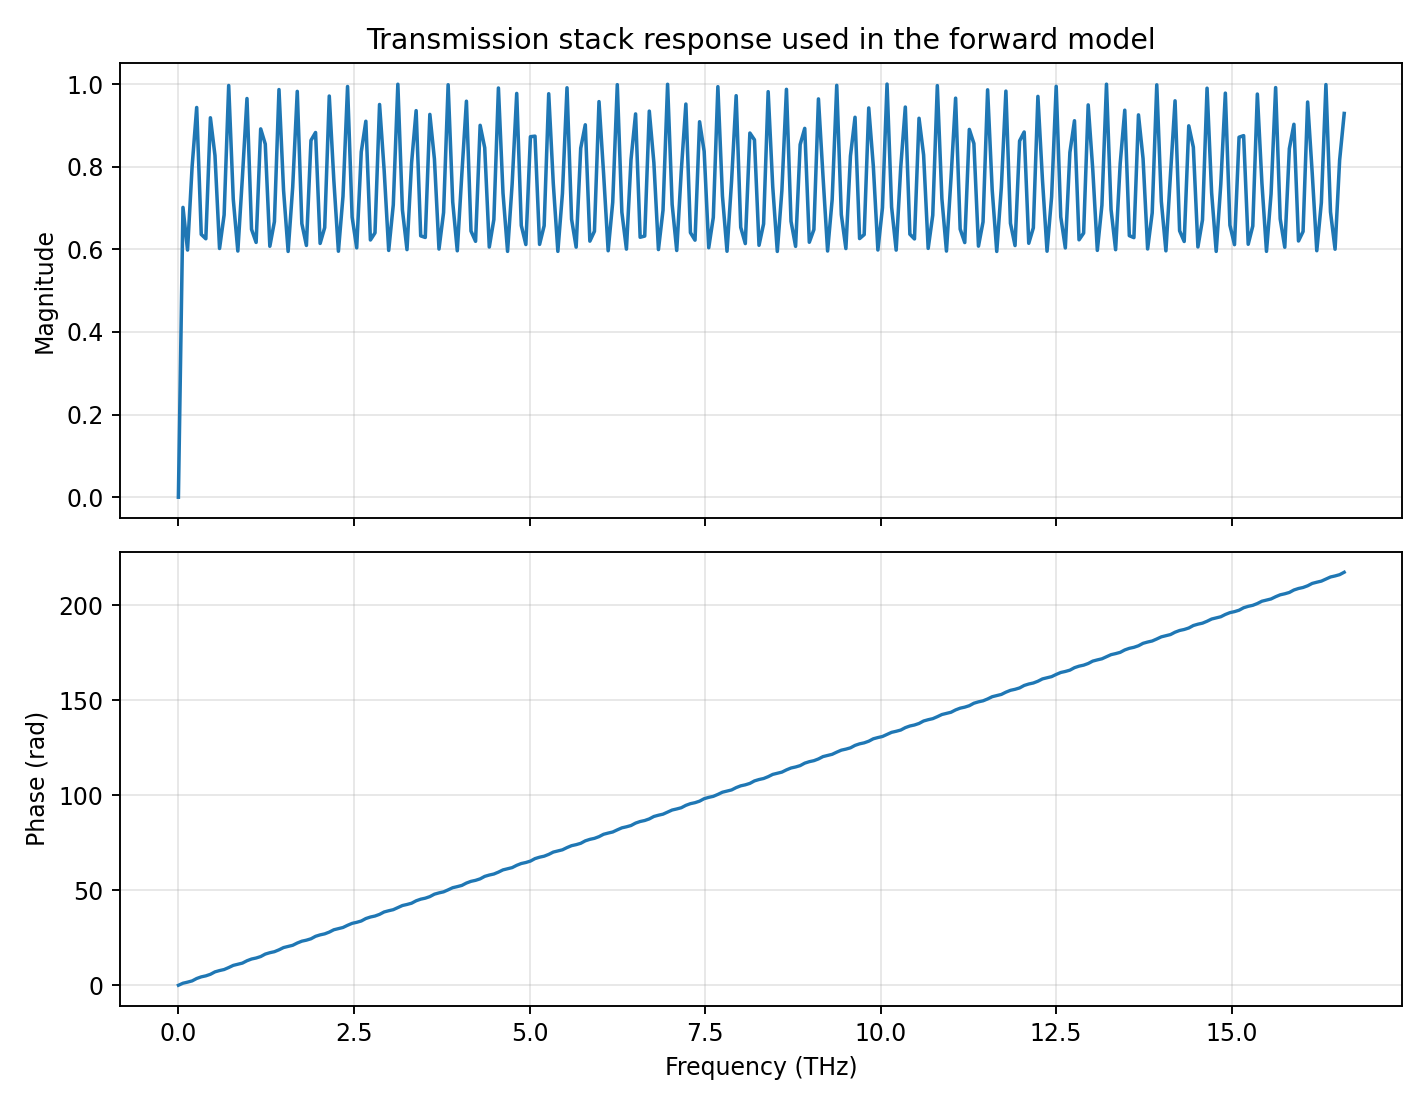
\includegraphics[width=0.82\linewidth]{transmission_stack_response.png}
\caption{Transmission worked example: the complex transfer function used in
\texttt{simulate\_sample\_from\_reference}.}
\end{figure}

\section{Forward Model with Measured Reference Normalization}
\subsection{Reference-standard normalization}
The central forward-model equation implemented in
\texttt{thzsim2/core/forward.py} is
\[
E_{\text{sam}}(\omega)
=
E_{\text{ref,meas}}(\omega)
\frac{H_{\text{sample}}(\omega)}
{H_{\text{ref,std}}(\omega)}.
\]
This is exactly the physical assumption used in the user plan:
\begin{itemize}[leftmargin=2em]
\item the measured reference trace contains the PCA source spectrum, detector response, and
common-path optics,
\item the modeled sample-plane response is factored in through
$H_{\text{sample}} / H_{\text{ref,std}}$,
\item the reference standard may be the identity or an explicit physical stack.
\end{itemize}

\subsection{Implementation details}
\texttt{simulate\_sample\_from\_reference(...)} performs
\begin{enumerate}[leftmargin=2em]
\item \texttt{fft\_t\_to\_w} on the reference trace,
\item \texttt{stack\_response\_function(...)} on the sample stack,
\item the same stack-response calculation on the reference-standard stack if one is supplied,
\item the ratio
$H_{\text{sample}}/H_{\text{ref,std}}$,
\item multiplication by the measured reference spectrum,
\item \texttt{ifft\_w\_to\_t} back to the time domain.
\end{enumerate}

Reflection measurements have no silent default reference standard. This is enforced by
\texttt{normalize\_measurement(...)}. The helper
\texttt{\_validate\_reference\_standard\_response(...)} also rejects normalization cases where
$H_{\text{ref,std}}(\omega)$ becomes numerically too small.

\section{Time-Domain Fitting}
\subsection{Parameter mapping}
The fitter works on a flat vector
\[
\mathbf{x} = (x_1,\dots,x_p),
\]
but the simulator requires a nested resolved-stack dictionary. The helper functions
\texttt{\_parse\_path}, \texttt{\_get\_by\_path}, \texttt{\_set\_by\_path},
\texttt{stack\_path\_from\_user\_path}, and \texttt{apply\_fit\_values} perform the algebraic
mapping
\[
\mathbf{x} \longrightarrow \text{resolved stack}.
\]

\subsection{Synthetic observations and noise}
For study runs and documentation examples, the code adds white Gaussian noise through
\texttt{add\_white\_gaussian\_noise(...)}. The standard deviation is derived from the requested
dynamic range by
\[
\sigma_{\text{noise}}
=
\frac{\max_t |E_{\text{sam,true}}(t)|}{10^{D/20}},
\]
where $D$ is the dynamic range in dB. This is implemented by
\texttt{noise\_sigma\_from\_dynamic\_range(...)}.

\subsection{Objective function}
The primary time-domain objectives are
\[
\mathrm{MSE}
=
\frac{1}{N}\sum_{n=0}^{N-1}
\left(
E_{\text{model}}(t_n)-E_{\text{obs}}(t_n)
\right)^2,
\]
and
\[
\mathrm{relative}\ L^2
=
\frac{\lVert E_{\text{model}}-E_{\text{obs}}\rVert_2}
{\max(\lVert E_{\text{obs}}\rVert_2,10^{-30})}.
\]
The selector \texttt{objective\_metric\_value(...)} chooses between them. The diagnostic
\texttt{snr\_db(...)} uses
\[
\mathrm{SNR}_{\mathrm{dB}}
=
20 \log_{10}
\left(
\frac{\mathrm{RMS}(E_{\text{signal}})}{\mathrm{RMS}(E_{\text{noise}})}
\right).
\]

\subsection{Optimization sequence}
\texttt{fit\_sample\_trace(...)} uses a two-stage search:
\begin{enumerate}[leftmargin=2em]
\item bounded differential evolution,
\item bounded local refinement with \texttt{L-BFGS-B}.
\end{enumerate}
Each trial vector $\mathbf{x}$ is mapped into a stack, simulated by
\texttt{simulate\_sample\_from\_reference(...)} with the current \texttt{Measurement}, and
scored in the time domain.

\subsection{Residual vector and covariance estimate}
After the optimum $\hat{\mathbf{x}}$ is found, the code builds the residual vector
\[
\mathbf{r}(\mathbf{x}) = E_{\text{obs}} - E_{\text{model}}(\mathbf{x}).
\]
\texttt{\_residual\_vector(...)} concatenates real and imaginary parts only if the residual is
complex; for the usual real time-domain fit, it remains a real vector of length $N$.

The finite-difference Jacobian used by \texttt{\_estimate\_parameter\_sigmas(...)} is
\[
J_{:,j}
\approx
\frac{
\mathbf{r}(\hat{\mathbf{x}}+\Delta x_j \mathbf{e}_j)
-
\mathbf{r}(\hat{\mathbf{x}}-\Delta x_j \mathbf{e}_j)
}
{
(\hat{x}_j+\Delta x_j)-(\hat{x}_j-\Delta x_j)
}.
\]
The step length is chosen by \texttt{\_step\_from\_bounds(...)} from the parameter magnitude,
the fit span, and the configured relative finite-difference step.

With $m$ residual samples and $p$ fitted parameters,
\[
\hat{\sigma}^2 = \frac{\mathbf{r}^T \mathbf{r}}{\max(m-p,1)},
\qquad
\Sigma \approx \hat{\sigma}^2 (J^T J)^+,
\]
where $(\cdot)^+$ is the pseudoinverse. The reported standard deviations and correlations are
\[
\sigma_j = \sqrt{\Sigma_{jj}},
\qquad
\rho_{ij} = \frac{\Sigma_{ij}}{\sigma_i \sigma_j}.
\]

\section{Edge Cases and Constraints}
\begin{itemize}[leftmargin=2em]
\item \textbf{Isotropic only.} The code assumes scalar $\tilde{n}(\omega)$ in each layer.
\item \textbf{One measured channel per run.} Each fit uses one geometry and one polarization
channel.
\item \textbf{Reflection requires an explicit standard.} This is enforced by
\texttt{normalize\_measurement(...)}.
\item \textbf{Empty stack is a direct interface.} If $n_{\text{in}} \neq n_{\text{out}}$, a
layer-free stack still has nontrivial Fresnel response.
\item \textbf{Zero-thickness limit collapses to the direct interface.} This is handled in
\texttt{single\_layer\_transfer(...)}.
\item \textbf{Normal incidence collapses \texttt{s}/\texttt{p}.} The reported reflected
\texttt{p} convention is chosen so the scalar channel is degenerate at $\theta_0=0$.
\item \textbf{Single-layer finite reflection count.} The explicit integer
\texttt{max\_internal\_reflections} truncation is exact for one layer. General multilayers use
the exact coherent recursion.
\item \textbf{Passive branch selection.} \texttt{nk\_from\_eps(...)} enforces $k \ge 0$.
\end{itemize}

\section{Worked Example A: Transmission Time-Domain Fit}
The documentation figure script \texttt{docs/generate\_time\_domain\_fit\_figures.py} builds a
Drude film with these true values:
\[
d = \SI{182}{\micro\meter},
\qquad
\tau = \SI{5.2}{\pico\second},
\qquad
\sigma = \SI{2.8e-2}{\siemens\per\meter},
\]
at
\[
\theta_0 = 30^\circ,
\qquad
\texttt{polarization}=\texttt{p},
\qquad
\texttt{mode}=\texttt{transmission}.
\]
The notebook-facing fit variables are thickness, Drude plasma frequency, and Drude damping
frequency. The clean simulated sample trace is generated by
\[
E_{\text{sam,true}}(\omega)
=
E_{\text{ref}}(\omega) H_{\text{sample}}(\omega),
\]
Gaussian noise is added at \SI{85}{dB} dynamic range, and the fit then minimizes the time-domain
MSE.

\begin{figure}[htbp]
\centering
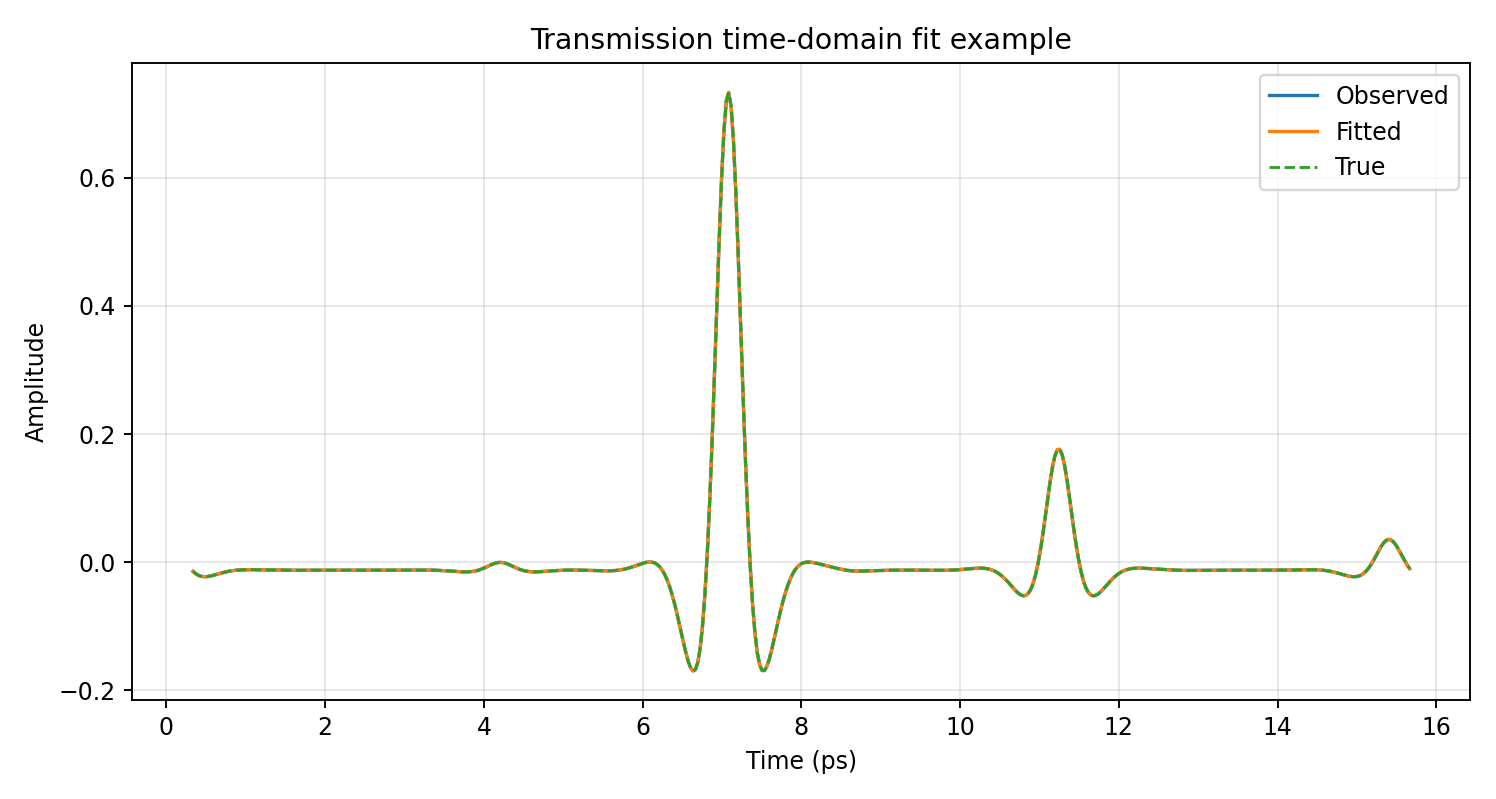
\includegraphics[width=0.82\linewidth]{transmission_time_fit.png}
\caption{Transmission worked example: noisy observed trace, true trace, and recovered fitted
trace.}
\end{figure}

\begin{figure}[htbp]
\centering
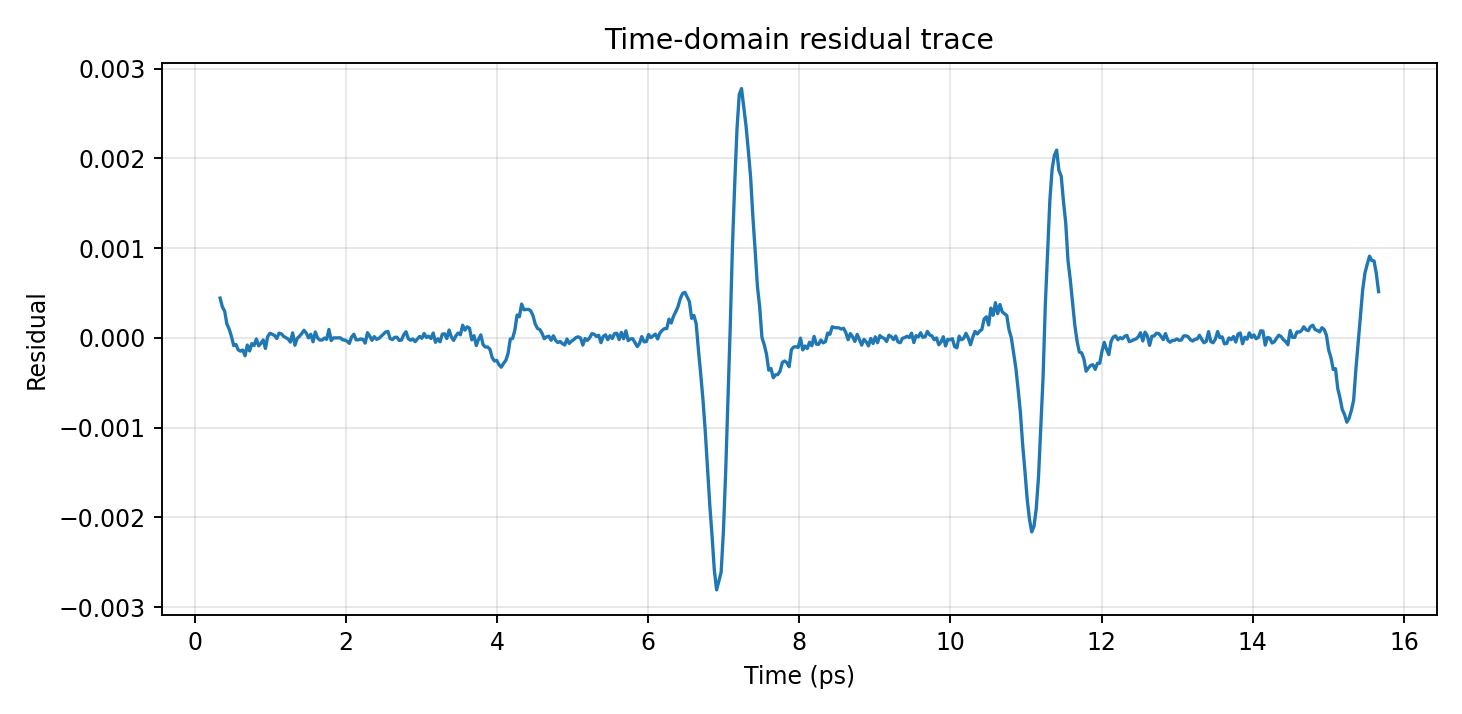
\includegraphics[width=0.82\linewidth]{transmission_residual.png}
\caption{Residual trace from the transmission worked example.}
\end{figure}

\paragraph{Algebraic structure of the fit.}
For each optimizer call:
\begin{enumerate}[leftmargin=2em]
\item \texttt{apply\_fit\_values(...)} writes $\mathbf{x}$ into the resolved stack.
\item \texttt{stack\_response\_function(...)} computes $H_{\text{sample}}(\omega)$.
\item \texttt{simulate\_sample\_from\_reference(...)} produces $E_{\text{model}}(t)$.
\item \texttt{objective\_metric\_value(...)} compares $E_{\text{model}}(t)$ to
$E_{\text{obs}}(t)$.
\end{enumerate}
This is repeated inside differential evolution and then inside the local bounded minimizer.

\section{Worked Example B: Reflection with Explicit Reference Standard}
The reflection example in the figure script uses
\[
\theta_0 = 45^\circ,
\qquad
\texttt{polarization}=\texttt{s},
\qquad
\texttt{mode}=\texttt{reflection},
\]
for a thin coating above an exit half-space with
\[
n_{\text{out}} = 1.52.
\]
The reference standard is the bare interface itself, represented as an explicit stack with no
physical layers and \texttt{n\_out = 1.52}. The forward model therefore uses
\[
E_{\text{sam}}(\omega)
=
E_{\text{ref,meas}}(\omega)
\frac{H_{\text{coated interface}}(\omega)}
{H_{\text{bare interface}}(\omega)}.
\]

\begin{figure}[htbp]
\centering
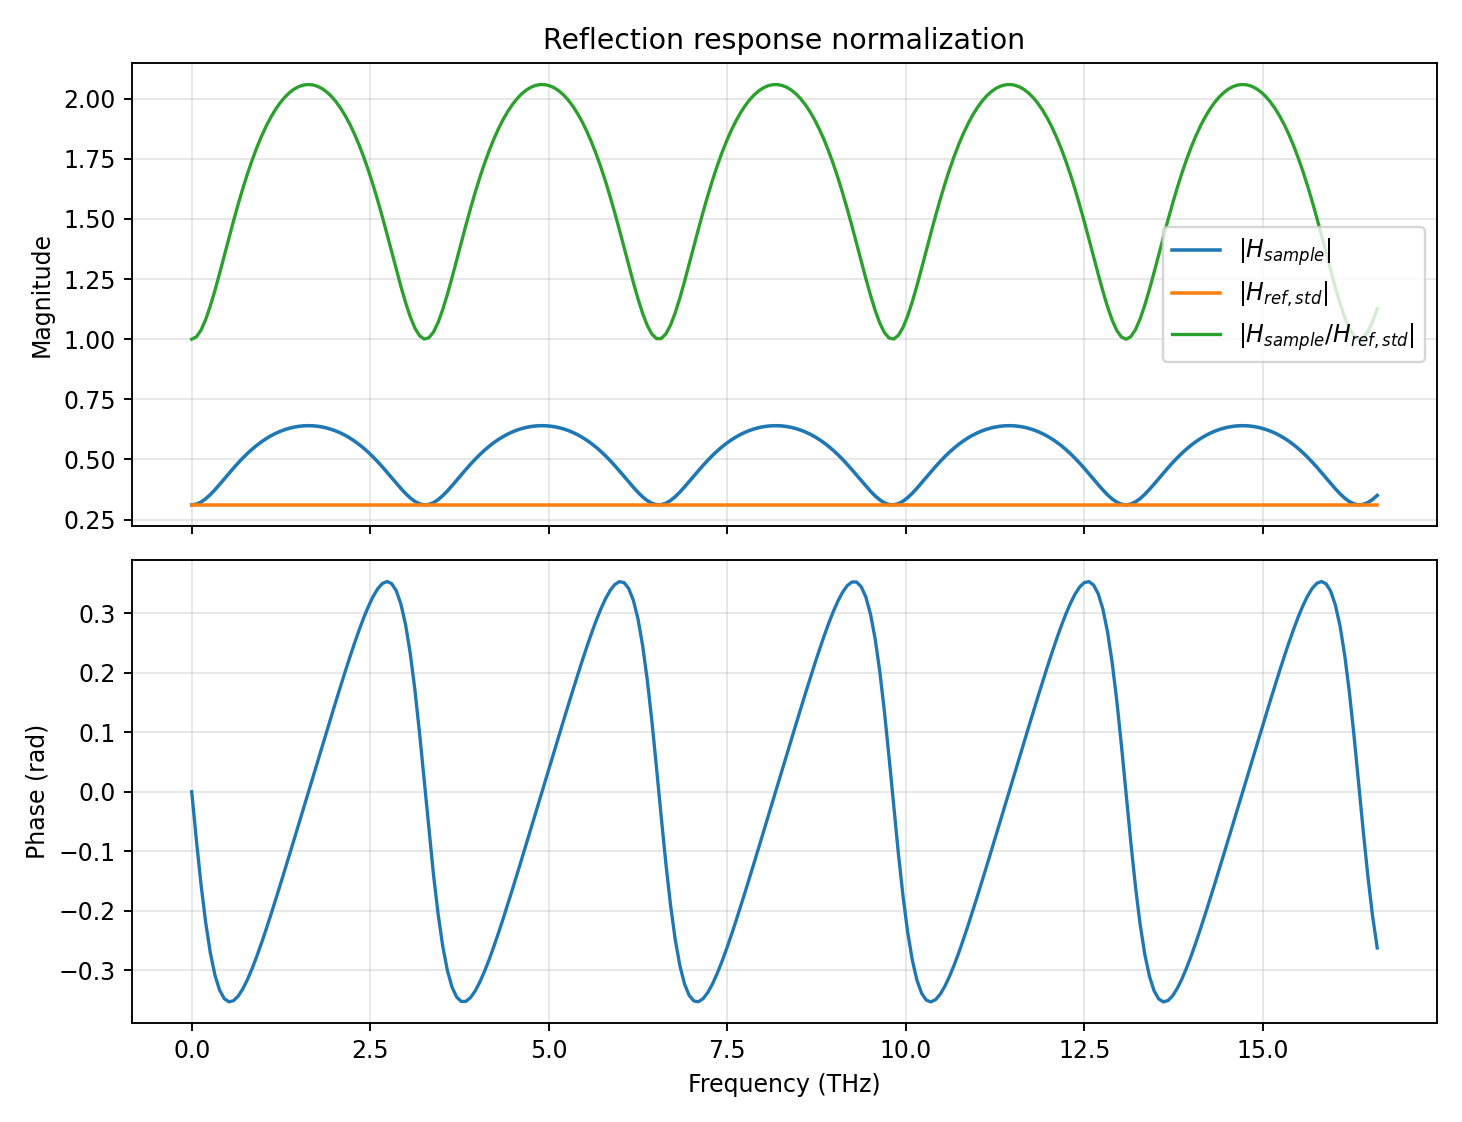
\includegraphics[width=0.82\linewidth]{reflection_normalized_response.png}
\caption{Reflection worked example: sample response, reference-standard response, and their
ratio.}
\end{figure}

\begin{figure}[htbp]
\centering
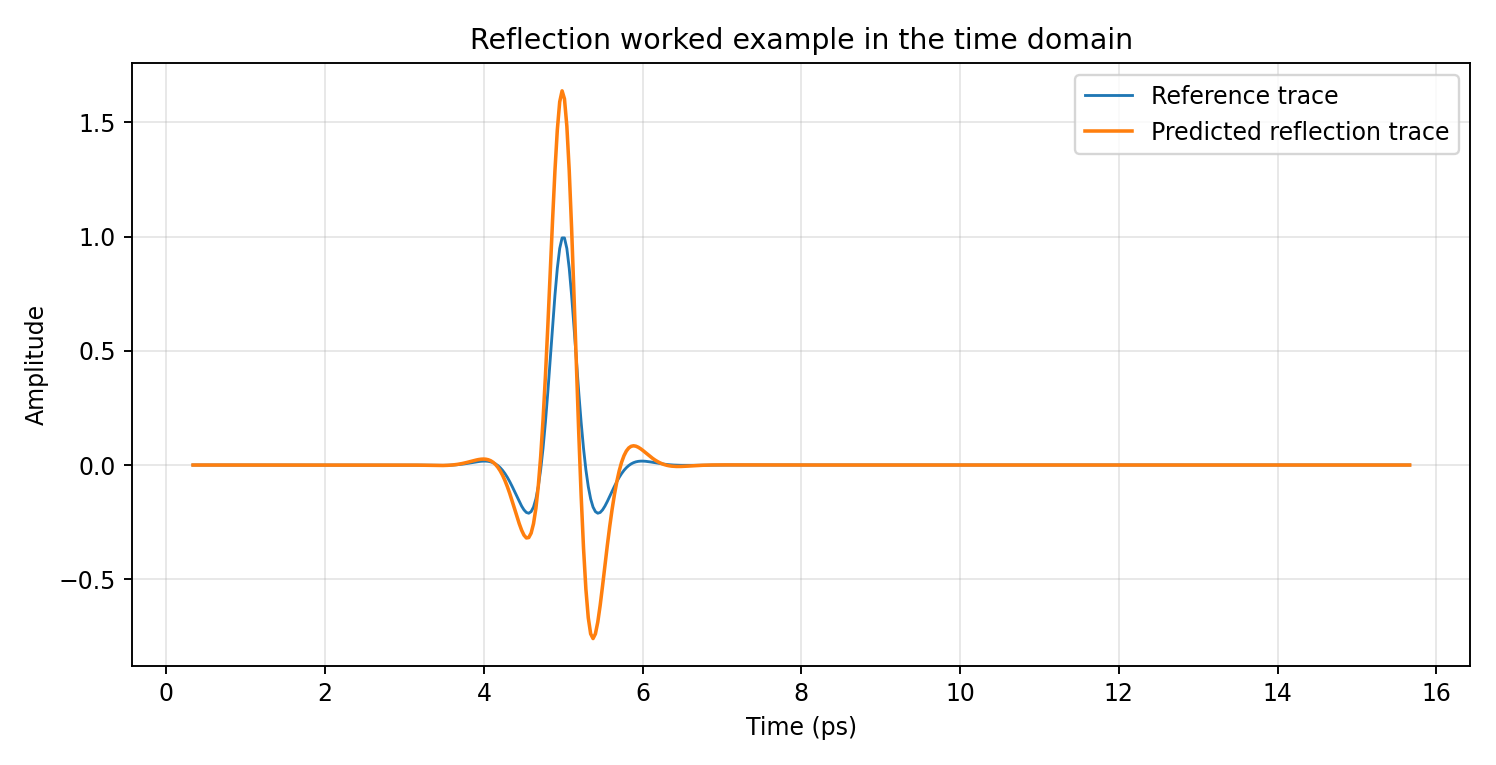
\includegraphics[width=0.82\linewidth]{reflection_time_trace.png}
\caption{Reflection worked example in the time domain.}
\end{figure}

\section{Code Crosswalk}
\renewcommand{\arraystretch}{1.2}
\begin{longtable}{p{0.30\linewidth} p{0.25\linewidth} p{0.35\linewidth}}
\toprule
\textbf{Calculation block} & \textbf{Primary functions} & \textbf{Role in the pipeline} \\
\midrule
\endfirsthead
\toprule
\textbf{Calculation block} & \textbf{Primary functions} & \textbf{Role in the pipeline} \\
\midrule
\endhead
Reference generation / import &
\texttt{generate\_reference\_pulse}, \texttt{load\_reference\_csv}, \texttt{prepare\_reference} &
Construct the measured or synthetic reference trace and its exported summary. \\

Time and frequency grids &
\texttt{make\_time\_grid}, \texttt{make\_omega\_grid}, \texttt{fft\_t\_to\_w}, \texttt{ifft\_w\_to\_t} &
Define the discrete Fourier convention used by the forward model and inverse synthesis. \\

Pulse models &
\texttt{gaussian\_carrier\_pulse}, \texttt{sech\_carrier\_pulse}, \texttt{make\_pulse} &
Generate the analytic source waveform when the reference is synthetic. \\

Material permittivity models &
\texttt{eps\_drude}, \texttt{eps\_lorentz}, \texttt{eps\_drude\_lorentz} &
Evaluate $\varepsilon(\omega)$ for supported isotropic material models. \\

Passive index extraction &
\texttt{nk\_from\_eps}, \texttt{evaluate\_material\_nk}, \texttt{\_nk\_from\_material\_dict} &
Convert dielectric functions into $n(\omega)$ and $k(\omega)$ on the working grid. \\

Sample resolution &
\texttt{build\_sample}, \texttt{\_resolve\_material}, \texttt{\_resolve\_value} &
Turn notebook-facing sample definitions into a resolved simulation stack and fit registry. \\

Oblique-interface optics &
\texttt{fresnel\_t\_oblique}, \texttt{fresnel\_r\_oblique}, \texttt{\_forward\_cos\_theta} &
Compute angle-aware interface amplitudes with a stable branch choice in complex media. \\

Layer propagation &
\texttt{propagation\_factor}, \texttt{\_propagation\_factor\_oblique} &
Apply the phase / attenuation factor across each layer. \\

Finite single-layer Fabry--Perot series &
\texttt{\_finite\_fp\_factor}, \texttt{\_medium\_stack\_response\_positive} &
Evaluate explicitly truncated round-trip sums when a single layer requests a finite count. \\

Exact multilayer response &
\texttt{\_multilayer\_response\_recursive}, \texttt{stack\_response\_function} &
Compute the exact coherent transmission or reflection of arbitrary isotropic multilayers. \\

Measurement normalization &
\texttt{Measurement}, \texttt{ReferenceStandard}, \texttt{normalize\_measurement}, \texttt{\_reference\_standard\_stack} &
Attach geometry, polarization, and reference-standard meaning to the forward model. \\

Forward simulation &
\texttt{simulate\_sample\_from\_reference} &
Apply $H_{\text{sample}}/H_{\text{ref,std}}$ to the measured reference and return the modeled trace. \\

Noise injection &
\texttt{noise\_sigma\_from\_dynamic\_range}, \texttt{add\_white\_gaussian\_noise} &
Generate synthetic noisy observations for studies and documentation examples. \\

Fit-parameter path mapping &
\texttt{\_parse\_path}, \texttt{\_get\_by\_path}, \texttt{\_set\_by\_path}, \texttt{stack\_path\_from\_user\_path}, \texttt{apply\_fit\_values} &
Map the optimizer vector into the nested resolved stack. \\

Objective and metrics &
\texttt{objective\_metric\_value}, \texttt{mse}, \texttt{relative\_l2}, \texttt{snr\_db} &
Score each simulated trace against the observed trace. \\

Optimization &
\texttt{fit\_sample\_trace} &
Run differential evolution plus bounded local refinement. \\

Local covariance estimate &
\texttt{\_residual\_vector}, \texttt{\_step\_from\_bounds}, \texttt{\_estimate\_parameter\_sigmas}, \texttt{\_correlation\_from\_covariance} &
Approximate local uncertainties and parameter correlations from a finite-difference Jacobian. \\
\bottomrule
\end{longtable}

\section{Literature Anchors Used for the Implementation}
The implementation decisions in this refactor were cross-checked against the local PDF set in
\texttt{C:\textbackslash Users\textbackslash cs7bp\textbackslash Desktop\textbackslash THz\_application\_sim - Copy}.
The most relevant anchors were:
\begin{itemize}[leftmargin=2em]
\item \textbf{\texttt{diss\_hoffmann.pdf}}: PCA emission is strongly linearly polarized, which
supports the single measured scalar channel used here.
\item \textbf{\texttt{s10762-024-01011-x.pdf}}: oblique-incidence THz analysis requires explicit
\texttt{s}/\texttt{p} handling and careful reference treatment.
\item \textbf{\texttt{THz-TDS\_Time-Trace\_Analysis\_for\_the\_Extraction\_of\_Material\_and\_Metamaterial\_Parameters.pdf}}
and \textbf{\texttt{1810.12567v4 (1).pdf}}: time-trace fitting is a natural and physically
meaningful objective for THz-TDS.
\item \textbf{\texttt{s10762-025-01052-w.pdf}} and related THz-TDS transform notes: Fourier
convention, phase handling, and time-origin bookkeeping matter for robust fitting.
\end{itemize}

\end{document}
